\ifdefined\COMPLETE
\else
	\documentclass[10pt,twoside]{extarticle}

\usepackage{xcolor}

\usepackage{graphicx}

\usepackage{multicol}

\usepackage{background}

\usepackage{adjustbox}

\usepackage{ifoddpage}

%\usepackage{showframe}

\usepackage{fontspec}
\setmainfont{DejaVu Sans}
\setlength{\lefthyphenmin}{8}
\setlength{\righthyphenmin}{8}

\ifdefined\bleed
	\usepackage[paperheight=216mm, paperwidth=151mm, top=2.25cm, bottom=2.8cm, outer=1.1cm, inner=0.8cm,heightrounded,marginparwidth=0cm,marginparsep=0cm]{geometry}
\else
	\usepackage[paperheight=210mm, paperwidth=148mm, top=1.95cm, bottom=2.5cm, outer=0.8cm, inner=0.8cm,heightrounded,marginparwidth=0cm,marginparsep=0cm]{geometry}
\fi

\newcommand{\getdefaultbggraphic}{
	\ifdefined\nobackground
	\else
		\checkoddpage
		\ifdefined\bleed
			\ifoddpage
		   		
\includegraphics[trim = 0 0 0 0,clip,width = \paperwidth,height = \paperheight, keepaspectratio]{images/songbackground_right.pdf}
			\else
		   		
\includegraphics[trim = 0 0 0 0,clip,width = \paperwidth,height = \paperheight, keepaspectratio]{images/songbackground_left.pdf}
			\fi
		\else
			\ifoddpage
		   		
\includegraphics[trim = 0 3mm 3mm 3mm,clip,width = \paperwidth,height = \paperheight, keepaspectratio]{images/songbackground_right.pdf}
			\else
		   		
\includegraphics[trim = 3mm 3mm 0 3mm,clip,width = \paperwidth,height = \paperheight, keepaspectratio]{images/songbackground_left.pdf}
			\fi
		\fi
	\fi
}

\setlength{\parskip}{0em} 
\setlength{\parindent}{0em}
\setlength{\columnsep}{0.3cm}
\setlength{\columnseprule}{0.5pt}

\usepackage{fancyhdr}
\fancypagestyle{song} {
	\fancyhead[L]{\vspace*{1em}\makesongheader}
	\fancyhead[R]{\makesongcredits}
	\fancyfoot{}
	\fancyfoot[C]{\makebox[\textwidth][c]{--- {\thepage} ---}}
	\fancyhfoffset[r]{\dimexpr+0.2cm\relax}
	\renewcommand{\headrulewidth}{0pt}
	\renewcommand{\footrulewidth}{0pt}
	\setlength{\headheight}{35pt}
	\backgroundsetup{opacity = 1, scale = 1, angle = 0,
	   contents = {\getdefaultbggraphic}}
}
\fancypagestyle{default} {
	\fancyhead{}
	\fancyhead[L]{\ifdefined\pagetitletext\vspace*{1em}\pagetitle{\pagetitletext}\\\fi}
	\fancyfoot{}
	\fancyfoot[C]{\makebox[\textwidth][c]{--- {\thepage} ---}}
	\renewcommand{\headrulewidth}{0pt}
	\renewcommand{\footrulewidth}{0pt}
	\setlength{\headheight}{35pt}
	\backgroundsetup{opacity = 1, scale = 1, angle = 0,
	   contents = {\getdefaultbggraphic}}
}
\fancypagestyle{nopagenum} {
	\fancyhead{}
	\fancyfoot{}
	\renewcommand{\headrulewidth}{0pt}
	\renewcommand{\footrulewidth}{0pt}
	\setlength{\headheight}{35pt} 
}
\fancypagestyle{empty} {
	\fancyhead{}
	\fancyfoot{}
	\renewcommand{\headrulewidth}{0pt}
	\renewcommand{\footrulewidth}{0pt}
	\setlength{\headheight}{0pt} 
	\backgroundsetup{contents = {}}
}
\pagestyle{default}

\title{Aqours 3rd Live WONDERFUL STORIES - Unofficial Information Booklet}
\author{Suyooo}
\date{July 15, 2018}

\newcommand{\fullimagepage}[2]{
	\newpage
	\thispagestyle{nopagenum}
	\ifdefined\nobackground
		\backgroundsetup{contents = {}}
		\vspace*{\fill}
		\vspace{-5em}
		\begin{center}#2\end{center}
		\vspace{\fill}
	\else
		\backgroundsetup{opacity = 1, scale = 1, angle = 0,
			contents = {
				\ifdefined\bleed
					\includegraphics[trim = 0 0 0 0,
					width = \paperwidth,
					height = \paperheight, keepaspectratio]
					{images/#1.png}
				\else
					\includegraphics[trim = 0 3mm 3mm 3mm,
					width = \paperwidth,
					height = \paperheight, keepaspectratio]
					{images/#1.png}
				\fi
			}}
		~\vfill
	\fi
	\newpage
	\backgroundsetup{opacity = 1, scale = 1, angle = 0,
	   contents = {\getdefaultbggraphic}}
}

\definecolor{chika}{HTML}{F0A20B}
\definecolor{riko}{HTML}{E9A9E8}
\definecolor{kanan}{HTML}{13E8AE}
\definecolor{dia}{HTML}{F23B4C}
\definecolor{you}{HTML}{49B9F9}
\definecolor{yohane}{HTML}{898989}
\definecolor{hanamaru}{HTML}{E6D617}
\definecolor{mari}{HTML}{AE58EB}
\definecolor{ruby}{HTML}{FB75E4}
\definecolor{aqours}{HTML}{3299E9}
\definecolor{sarah}{HTML}{3BB7EB}
\definecolor{leah}{HTML}{98ADD8}

\definecolor{clap}{HTML}{00CC22}
\definecolor{special}{HTML}{DDAA00}

\usepackage{shadowtext}
\shadowoffset{2pt}
\shadowcolor{black!5!white}

% ALTERNATING LETTER COLORS from https://tex.stackexchange.com/a/285974
\ExplSyntaxOn
\NewDocumentCommand{\colorstring}{O{aqours!90!white,aqours!95!black}+m}{%
  \clist_set:Nn \l_tmpa_clist {#1}%
  \int_zero:N \l_tmpa_int%
  \str_set:Nx \l_tmpa_str {#2}%
  \int_step_inline:nnnn {1} {1} {\str_count:N \l_tmpa_str } {%
    \str_case_x:nnF {\str_item:Nn \l_tmpa_str {##1}} {%
      {\space}{\space}
    }{%
      \int_compare:nNnTF {\l_tmpa_int } < {\clist_count:N \l_tmpa_clist } {
        \int_incr:N \l_tmpa_int
      }{%
        \int_set:Nn \l_tmpa_int {\c_one}
      }
      \textcolor{\clist_item:Nn \l_tmpa_clist {\l_tmpa_int }}{\hspace{-0.43em}\shadowtext{\str_item:Nn \l_tmpa_str {##1}}}
    }
  }
}
\ExplSyntaxOff

\newcommand{\call}[1]{{\textbf{\footnotesize{\textcolor{red}{(#1)}}}}}
\newcommand{\calltext}[1]{{\textbf{\textcolor{red}{#1}}}}
\newcommand{\callside}[1]{\hfill\call{#1}}
\newcommand{\callline}[1]{\vspace{-0.83em}\call{#1}\vspace{0.5em}}
\newcommand{\clap}[1]{{\textbf{\footnotesize{\textcolor{clap}{(#1)}}}}}
\newcommand{\clapline}[1]{\vspace{-0.83em}\clap{#1}\vspace{0.5em}}
\newcommand{\claptext}[1]{{\textbf{\textcolor{clap}{#1}}}}
\newcommand{\specinst}[1]{{\textbf{\footnotesize{\textcolor{special}{(#1)}}}}}
\newcommand{\specinstline}[1]{\vspace{-0.83em}\clap{#1}\vspace{0.5em}}
\newcommand{\specinsttext}[1]{{\textbf{\textcolor{special}{#1}}}}
\newcommand{\sing}[1]{{\textbf{\textcolor{aqours}{#1}}}}
\newcommand{\memberbg}[2]{\setlength{\fboxsep}{0pt}\colorbox{#1!30}{\makebox[\linewidth][l]{\strut{#2}}}}
\newcommand{\memberbgnote}[3]{{\footnotesize{\textcolor{#1}{\textbf{#3}}}}\\\memberbg{#1}{#2}}
\newcommand{\memberbgside}[3]{\memberbg{#1}{\strut{#2\hfill{\footnotesize{\textcolor{#1}{\textbf{#3}}}}}}}


\newcommand{\pagetitle}[1]{%
	\shadowcolor{aqours!25!white}%
	{\LARGE\textbf{\strut{\colorstring{#1}}}}%
	\shadowcolor{black!5!white}%
}

\newcommand{\cancel}[2]{%
    \tikz[baseline=(tocancel.base)]{
        \node[inner sep=0pt,outer sep=0pt] (tocancel) {#1};
        \node[red] at (0,0.66) {#2};
        \draw[line width=1mm, red] (tocancel.south west) -- (tocancel.north east);
    }%
}%

\def\changemargin#1#2{\list{}{\leftmargin#1\rightmargin#2}\item[]}
\let\endchangemargin=\endlist

\newcommand{\makesongheader}{
	\pagetitle{\songtitle}\\
	{\small\color{black!40!aqours}{\textbf{\songcomment}}}
}
\newcommand{\makesongcredits}{
	\adjustbox{scale={0.85}{1}}{\scriptsize{
		\color{black!40!aqours}{Writer \textbf{\songwriter} Lyrics \textbf{\songlyrics} Arrangement \textbf{\songarrange}}
	}}
}

\usepackage[hidelinks]{hyperref}

\ifdefined\COMPLETE
	\graphicspath{{./}}
\else
	\graphicspath{{../}}
\fi

	\begin{document}
\fi

\def\pagetitletext{Calls and Responses}
\newcommand{\aka}[2]{%
	\llap{\footnotesize\raisebox{-1.33em}{\textcolor{#1}{\textbf{aka #2}}\hspace{0.5em}}}%
}
\newcommand{\crdiv}[3]{
	\hspace*{1.35em}\tikz[baseline=(content.base)]{
	\begin{scope}[local bounding box=content]
		\node[text width=6.5cm-2em,minimum width=6.5cm,inner sep=1em,outer sep=0pt,right=0cm,align=justify] {{#3 \par}};
		\node[text width=6.5cm-2em,minimum width=6.5cm,inner sep=1em,outer sep=0pt,anchor=east] {\textbf{#2}};
	\end{scope}
	\draw[line width=1mm, transform canvas={xshift=0pt}, #1] (content.south west) -- (content.north west);
	}
	\vspace{1em}
}
\textbf{Calls and Responses} are used by the performers to introduce themselves. They will ask the audience to join them during the first MC. Here is a list of them, along with some translations and trivia!\\
Colored parts of each C\&R are the ones called by the performer, the black parts are the audience's response. Feel free to join in!\\
\vspace{\fill}\\

\includegraphics[width=2.7em,keepaspectratio]{images/icon_yohane.png}\raisebox{.66em}{
	\textbf{\LARGE\colorstring[yohane,yohane!75]{Aika Kobayashi}}\aka{yohane}{Aikyan} \colorstring[yohane]{as} \textbf{\large\cancel{\colorstring[yohane,yohane!75]{Yoshiko}}{Yohane} \colorstring[yohane!75,yohane]{Tsushima}}
}\\
\vspace{-1em}\\
\crdiv{yohane}{\textcolor{yohane}{Ohayohane!}\\Ohayoshiko!\\\textcolor{yohane}{Dakara Yohane yo!}\\Pyon--- {\normalfont\small (do a little hop)}}{\footnotesize The first two lines are puns on "Ohayou" ("good morning"). “Pyon” is a little harder to explain. It’s the onomatopoeia for a rabbit hopping, hence the hop.\\However, it’s also used in a cute, joking manner at the end of sentences, so a fitting translation would probably be "Oops, we did that by accident--- (we totally did it on purpose)"}
\vspace{\fill}\\

\includegraphics[width=2.7em,keepaspectratio]{images/icon_ruby.png}\raisebox{.66em}{
	\textbf{\LARGE\colorstring[ruby!95!black,ruby]{Ai Furihata}}\aka{ruby!95!black}{Furirin} \colorstring[ruby!95!black]{as} \textbf{\large\colorstring[ruby!95!black,ruby]{Ruby Kurosawa}}
}\\
\vspace{-1em}\\
\crdiv{ruby}{\textcolor{ruby!95!black}{Issho ni...}\\Ganbaruby!}{\footnotesize Of course, this C\&R includes the Ganbaruby pose, as seen in the anime.}
\vspace{\fill}\\

\includegraphics[width=2.7em,keepaspectratio]{images/icon_maru.png}\raisebox{.66em}{
	\textbf{\LARGE\colorstring[hanamaru!90!black,hanamaru!97!black]{Kanako Takatsuki}}\aka{hanamaru}{Kinchan} \colorstring[hanamaru]{as} \textbf{\large\colorstring[hanamaru!90!black,hanamaru!97!black]{Hanamaru Kunikida}}
}\\
\vspace{-1em}\\
\crdiv{hanamaru!95!black}{\textcolor{hanamaru!95!black}{Ohana...}\\Maru!\\ {\normalfont \small (form a circle above your head)}}{\footnotesize "Hanamaru" literally translates to "flower circle", which is why you make a circle on the "maru" part.}
\vspace{\fill}
\newpage

\vspace*{\fill}

\includegraphics[width=2.7em,keepaspectratio]{images/icon_riko.png}\raisebox{.66em}{
	\textbf{\LARGE\colorstring[riko!93!black,riko]{Rikako Aida}}\aka{riko!93!black}{Rikyako} \colorstring[riko!93!black]{as} \textbf{\large\colorstring[riko!93!black,riko]{Riko Sakurauchi}}
}\\
\vspace{-1em}\\
\crdiv{riko}{\textcolor{riko!85!black}{Beach sketch... \small\normalfont (Biichi suketchi)}\\Sakurauchi!\\\textcolor{riko!85!black}{Suki na tabemono wa...?}\\Sandwich! {\small\normalfont (Sandowichi)}\\\textcolor{riko!85!black}{Kurae!\\Riko-chan beeeam! \small\normalfont (biiimu)}}{\textbf{\textcolor{riko!85!black}{My favorite food is...?}\\Sandwiches!\\\textcolor{riko!85!black}{Take this! Riko Beeeam!}}\par\footnotesize This C\&R references Riko's neighborhood, hobby and favorite food (egg sandwiches). Rikyako only recently added the Riko Beam to her C\&R.}
\vspace{\fill}\\

\includegraphics[width=2.7em,keepaspectratio]{images/icon_chika.png}\raisebox{.66em}{
	\textbf{\LARGE\colorstring[chika,chika!75]{Anju Inami}}\aka{chika}{Anchan} \colorstring[chika]{as} \textbf{\large\colorstring[chika,chika!75]{Chika Takami}}
}\\
\vspace{-1em}\\
\crdiv{chika}{\textcolor{chika}{Kan Kan!}\\Mikan!\\\textcolor{chika}{Kan Kan!}\\Mikan!\\\textcolor{chika}{Kaaan Kaaan...}\\Mi-ka-n!}{\footnotesize "Mikan" is the japanese word for "tangerine". This C\&R was originally made for Anchan by Shukashuu and Furirin, her fellow CYaRon members, while she came up with the final, emphasized repeat.}
\vspace{\fill}\\

\includegraphics[width=2.7em,keepaspectratio]{images/icon_you.png}\raisebox{.66em}{
	\textbf{\LARGE\colorstring[you,you!75]{Shuka Saitou}}\aka{you}{Shukashuu} \colorstring[you]{as} \textbf{\large\colorstring[you,you!75]{You Watanabe}}
}\\
\vspace{-1em}\\
\crdiv{you}{\textcolor{you}{Zensoku zenshin...}\\Yousoro! {\normalfont\small (point to the stage)}\\\textcolor{you}{Kara no...}\\Keirei! {\normalfont\small (salute)}}{\textbf{\textcolor{you}{Full speed ahead...}\\Aye Aye!\\\textcolor{you}{And...}\\Salute!}}
\vspace{\fill}

\newpage
\vspace*{\fill}

\includegraphics[width=2.7em,keepaspectratio]{images/icon_kanan.png}\raisebox{.66em}{
	\textbf{\LARGE\colorstring[kanan!97!black,kanan!85]{Nanaka Suwa}}\aka{kanan}{Suwawa} \colorstring[kanan]{as} \textbf{\large\colorstring[kanan!97!black,kanan!85]{Kanan Matsuura}}
}\\
\vspace{-1em}\\
\crdiv{kanan}{\textcolor{kanan!90!black}{Minna-san,\\gokigen ika ga kanan?}\\Daibu ii kanji!\\\textcolor{kanan!90!black}{Yoshi -- jaa, hagu shiyou!}}{\textbf{\textcolor{kanan!90!black}{How is everyone doing?}\\We're feeling good!\\\textcolor{kanan!90!black}{Alright -- then let's hug!}}\par\footnotesize Several puns are hidden here: The call replaces "kana" with "Kanan", and the "daibu" in the response is also how "dive" is written in the Japanese syllabary.}
\vspace{\fill}\\

\includegraphics[width=2.7em,keepaspectratio]{images/icon_dia.png}\raisebox{.66em}{
	\textbf{\LARGE\colorstring[dia,dia!70]{Arisa Komiya}}\aka{dia}{Arisha} \colorstring[dia]{as} \textbf{\large\colorstring[dia,dia!70]{Dia Kurosawa}}
}\\
\vspace{-1em}\\
\crdiv{dia}{\textcolor{dia}{Daiyahoo!}\\Daiyahoo!\\\textcolor{dia}{Buu buu desu wa...}\\\normalfont{\small (repeat)}}{}
\vspace{\fill}\\

\includegraphics[width=2.7em,keepaspectratio]{images/icon_mari.png}\raisebox{.66em}{
	\textbf{\LARGE\colorstring[mari,mari!75]{Aina Suzuki}}\aka{mari}{Ainya} \colorstring[mari]{as} \textbf{\large\colorstring[mari,mari!75]{Mari Ohara}}
}\\
\vspace{-1em}\\
\crdiv{mari}{\textcolor{mari}{Minna-san, shiny!}\\Shiny!\\\textcolor{mari}{And... lock on!}\\{\normalfont \small (pretend to get shot)}}{}
\vspace{\fill}

\newpage

\vspace*{\fill}

\includegraphics[width=2.7em,keepaspectratio]{images/icon_sarah.png}\raisebox{.66em}{
	\textbf{\LARGE\colorstring[sarah,sarah!80]{Asami Tano}}\aka{sarah}{Asamin} \colorstring[sarah]{as} \textbf{\large\colorstring[sarah,sarah!80]{Sarah Kazuno}}
}\\
\vspace{-1em}\\
\crdiv{sarah}{\textcolor{sarah}{Gomen kudasaima-sarah!}\\Irrashaima-sarah!\\\textcolor{sarah}{Minna issho ni...}\\Yokkora-sarah!\\{\normalfont \small (do a squat, lift arms to the sides)}}{\footnotesize The C\&Rs of Saint Snow were suggested by fans in Uraraji. Leaving out the "Sarah" puns, this one translates to:\par\normalsize\textbf{\textcolor{sarah}{Excuse me!}\\Welcome!\\\textcolor{sarah}{Everyone together...}\\Heave-ho!}\par\footnotesize "Yokkorase" is an "expression of physical effort" -- another translation could be something like "alley-oop".}
\vspace{\fill}\\
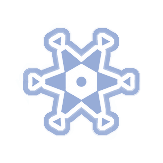
\includegraphics[width=2.7em,keepaspectratio]{images/icon_leah.png}\raisebox{.66em}{
	\textbf{\LARGE\colorstring[leah,leah!85]{Hinata Satou}}\aka{leah}{Hinahina} \colorstring[leah]{as} \textbf{\large\colorstring[leah,leah!85]{Leah Kazuno}}
}\\
\vspace{-1em}\\
\crdiv{leah}{\textcolor{leah}{Nee-sama no imouto wa...?}\\Kazuno Leah!\\\textcolor{leah}{Leah-chan power juuden dekitemasu ka?}\\Leah-juu!\\ {\normalfont \small (do the Saint Snow pose)}}{\textbf{\textcolor{leah}{Sarah's little sister is...?}\\Leah Kazuno!\\\textcolor{leah}{Is your Leah Power charged?}\\Fully charged!}\par\footnotesize "Leah-juu" is a combination of Leah's name and the "juu" from "juuden" (electrical charge) -- even though it's pronounced the same, it's unreleated to the well-known slang word "riajuu" ("normal person").}\\
\vspace{\fill}\\
{\small Saint Snow's C\&Rs are a little more involved - in case you have\\
trouble with them, check out Hinahina's video tutorial:\\
\textbf{\textcolor{aqours}{\hyperlink{https://twitter.com/satohina1223/status/989293745127358464}{twitter.com/satohina1223/status/989293745127358464}}}}
\vspace{-5.66em}\\
\hspace*{\fill}
\includegraphics[height=8em,keepaspectratio]{images/qr_hinahina_video.pdf}
\vspace{\fill}

\ifdefined\COMPLETE
\else
	\end{document}
\fi